\section{Iterative Refinement of Requirements}
\label{sec:requirements-evolution}

The requirements presented in the preceding sections were not specified in a single up-front pass.
Because a working prototype existed from the outset (\cref{sec:requirements-elicitation}), the platform was developed incrementally, and a substantial part of the requirement set emerged or was re-scoped as successive prototypes were demonstrated to the supervisors and reviewed against the research goals.
We make this refinement process explicit here for two reasons.
First, the design-time emergence of requirements is itself evidence that the elicitation method described in \cref{sec:requirements-elicitation} was functioning as intended, generalising the two emergent requirements (FR23 and FR24) already noted in Sec.~\ref{sec:functional-requirements}.
Second, the trajectory of the requirement set is part of the engineering record: it documents which capabilities were anticipated and which were discovered only by building the system and observing it in use.

We note one methodological caveat.
No formal requirements change-log was maintained during the early iterations; the refinement history reported in this section was reconstructed retrospectively from the project's version-control history and from supervision notes.
The reconstruction is therefore approximate in its timing, although the substantive changes it records are evidenced by the corresponding implementation work.
Each iteration followed the build--demonstrate--feedback--refine cycle of the development approach set out in \cref{ch:methodology}: a prototype increment was produced, demonstrated to the supervisors, discussed, and the resulting feedback was folded back into the requirement set before the next increment.
Refinements took three forms: a new capability was added, an existing requirement was re-scoped, or an approach that had been tried was abandoned and replaced.

\usetikzlibrary{arrows.meta}
\begin{figure}[htbp]
\centering
\resizebox{0.98\linewidth}{!}{%
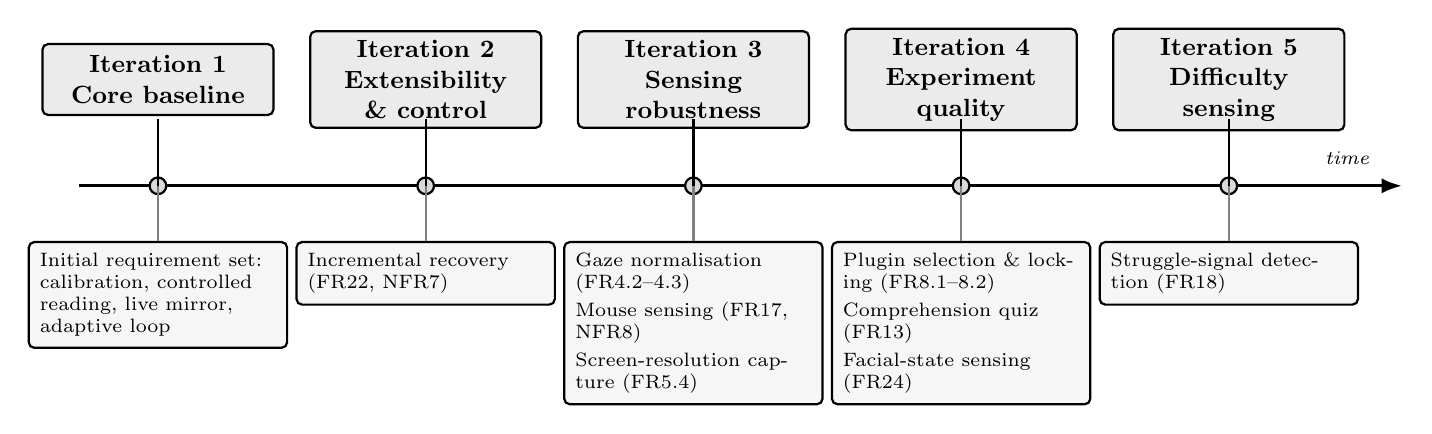
\begin{tikzpicture}[
  milestone/.style={circle, draw, thick, fill=gray!30, minimum size=6pt, inner sep=0pt},
  ittitle/.style={draw, thick, rounded corners=2pt, fill=gray!16, align=center,
                  text width=2.7cm, minimum height=0.9cm, font=\small\bfseries},
  reqbox/.style={draw, thick, rounded corners=2pt, fill=gray!7, align=left,
                 text width=3.0cm, font=\scriptsize, inner sep=4pt},
  axis/.style={-{Latex[length=2.6mm]}, very thick}
]

\def\xa{0} \def\xb{3.4} \def\xc{6.8} \def\xd{10.2} \def\xe{13.6}

\draw[axis] (-1.0,0) -- (\xe+2.2,0);
\node[anchor=west, font=\scriptsize\itshape] at (\xe+1.1,0.35) {time};

\foreach \x in {\xa,\xb,\xc,\xd,\xe} { \node[milestone] at (\x,0) {}; }

\node[ittitle] at (\xa,1.35) {Iteration 1\\Core baseline};
\node[ittitle] at (\xb,1.35) {Iteration 2\\Extensibility \& control};
\node[ittitle] at (\xc,1.35) {Iteration 3\\Sensing robustness};
\node[ittitle] at (\xd,1.35) {Iteration 4\\Experiment quality};
\node[ittitle] at (\xe,1.35) {Iteration 5\\Difficulty sensing};
\foreach \x in {\xa,\xb,\xc,\xd,\xe} { \draw[thick] (\x,0) -- (\x,0.85); }

\node[reqbox, anchor=north] at (\xa,-0.7)
  {Initial requirement set: calibration, controlled reading, live mirror, adaptive loop};
\node[reqbox, anchor=north] at (\xb,-0.7)
  {Incremental recovery (FR22, NFR7)};
\node[reqbox, anchor=north] at (\xc,-0.7)
  {Gaze normalisation (FR4.2--4.3)\\[2pt] Mouse sensing (FR17, NFR8)\\[2pt]
   Screen-resolution capture (FR5.4)};
\node[reqbox, anchor=north] at (\xd,-0.7)
  {Plugin selection \& locking (FR8.1--8.2)\\[2pt] Comprehension quiz (FR13)\\[2pt]
   Facial-state sensing (FR24)};
\node[reqbox, anchor=north] at (\xe,-0.7)
  {Struggle-signal detection (FR18)};
\foreach \x in {\xa,\xb,\xc,\xd,\xe} { \draw[thick, gray] (\x,0) -- (\x,-0.7); }

\end{tikzpicture}%
}
\caption[Timeline of the five development iterations.]{Timeline of the five development iterations and the requirements that emerged or were re-scoped in each.
Iteration~1 established the initial requirement set; subsequent iterations added or refined requirements in response to prototypes demonstrated to the supervisors.
Requirement identifiers refer to Tab.~\ref{tab:fr} and Tab.~\ref{tab:nfr}.}
\label{fig:requirements-evolution}
\end{figure}

Fig.~\ref{fig:requirements-evolution} summarises the five iterations and the requirements that emerged in each, and Tab.~\ref{tab:req-evolution} traces each refinement from the observation that triggered it to the resulting requirement.
Iteration~1 produced the core adaptive-reading baseline and the initial requirement set; the refinements of interest occur in the later iterations.

\begingroup
\small
\begin{longtable}{@{} p{0.05\linewidth} p{0.55\linewidth} p{0.32\linewidth} @{}}
\caption[Requirements that emerged or were re-scoped across iterations.]{Requirements that emerged or were re-scoped across development iterations, traced from the triggering observation to the resulting requirement. Identifiers refer to Tab.~\ref{tab:fr} and Tab.~\ref{tab:nfr}.}
\label{tab:req-evolution} \\
\toprule
\textbf{It.} & \textbf{Triggering observation} & \textbf{Resulting requirement(s)} \\
\midrule
\endfirsthead

\multicolumn{3}{c}{\tablename~\thetable{} --- continued} \\
\toprule
\textbf{It.} & \textbf{Triggering observation} & \textbf{Resulting requirement(s)} \\
\midrule
\endhead

\midrule
\multicolumn{3}{r}{\footnotesize Continued on next page} \\
\endfoot

\bottomrule
\endlastfoot

2 & An abrupt termination mid-session would lose all data collected up to that point. & Incremental session checkpointing and recovery (FR22, NFR7) \\[2pt]
3 & Raw gaze was too jittery for reliable word-level mapping, flickering between adjacent lines. & Coordinate normalisation and reading-line bias (FR4.2, FR4.3, FR5.4) \\[2pt]
3 & Tobii hardware was not always available for development, demonstration, or testing. & Mouse-cursor sensing mode and hardware-independent operation (FR17; NFR8; US-R5) \\[2pt]
3 & Word-level areas of interest are computed in pixels and therefore depend on the participant's display. & Capture of participant screen resolution for valid mapping (FR4.3, FR5.4) \\[2pt]
4 & Experiments require a fixed, reproducible module configuration per reading material. & Per-material decision and analysis plugin selection and locking (FR8.1, FR8.2; FR5.3) \\[2pt]
4 & Gaze indicates where a participant looks but not whether they comprehended the text. & End-of-reading comprehension quiz (FR13; US-R2, US-P3) \\[2pt]
4 & A signal beyond gaze was wanted to corroborate participant engagement. & Optional facial-state sensing module (FR24) \\[2pt]
5 & Interventions needed a difficulty signal derived from reading behaviour to act on. & Struggle-signal detection from fixation and saccade patterns (FR18) \\

\end{longtable}
\endgroup

Several of these refinements illustrate the value of the iterative approach.
The gaze stream produced by the early prototype was visibly unstable: a reader fixating mid-line produced samples that alternated between adjacent lines, which corrupted word-level attention mapping.
This observation motivated the coordinate normalisation and reading-line bias that stabilise the mapping (FR4.2, FR4.3, FR5.4), a heuristic we revisit critically in \cref{ch:discussion}.
A second refinement addressed the practical reality that Tobii hardware was not always available during development: this drove the mouse-cursor sensing mode (FR17) and the requirement that the platform remain fully operable without physical eye-tracking hardware (NFR8).
A third refinement followed from a measurement gap rather than a technical one: gaze data captures where a participant looks but not whether they understood the text, which motivated the optional comprehension quiz (FR13) so that reading effectiveness could be assessed alongside attention.

The clearest example of re-scoping concerns facial-state sensing.
A webcam was first introduced as an additional gaze \emph{input mode}, on the assumption that it could serve as a low-cost sensing source comparable to the eye tracker.
Demonstrating this increment showed the assumption to be unfounded: a webcam does not yield gaze of comparable quality, and forcing it into the sensing-mode abstraction conflated two different kinds of signal.
The input mode was therefore removed, and the capability re-entered the system in a different role, as an optional facial-state \emph{module} supplying supplementary engagement context through the external module-provider framework (FR24).
This episode is a concrete demonstration of the extensibility the architecture targets (NFR6): a capability could be withdrawn from one extension point and reintroduced at another without disturbing the core, and it is the reason FR24 carries a Could-have priority and an explicit independence clause.

Taken together, these refinements substantiate the iterative elicitation claim made in \cref{sec:requirements-elicitation} and show that the requirement set is grounded in demonstrated need rather than up-front speculation.
The requirements established across this chapter are nonetheless bounded by a number of fixed external constraints, which the next section makes explicit.
